\documentclass[twocolumn]{extarticle}
\usepackage{fontspec}   %加這個就可以設定字體
\usepackage{xeCJK}       %讓中英文字體分開設置

\usepackage{listings}
\usepackage[newfloat]{minted}
\usepackage{float}
\usepackage{graphicx}
\usepackage{caption}
\usepackage{fancyhdr}
\usepackage{hyperref}
\usepackage{amsmath}
\DeclareMathOperator*{\argmax}{arg\,max}
\DeclareMathOperator*{\argmin}{arg\,min}
\usepackage{multirow}
\usepackage[dvipsnames]{xcolor}
\usepackage{graphicx}
\usepackage{tabularx}
\usepackage{booktabs}
\usepackage{caption}
\usepackage{subcaption}
\usepackage{pifont}
\usepackage{amssymb}
\usepackage{titling}

\usepackage{pdftexcmds}
\usepackage{catchfile}
\usepackage{ifluatex}
\usepackage{ifplatform}

\usepackage[breakable, listings, skins, minted]{tcolorbox}
\usepackage{etoolbox}
\setminted{fontsize=\footnotesize}
\renewtcblisting{minted}{%
    listing engine=minted,
    minted language=python,
    listing only,
    breakable,
    enhanced,
    minted options = {
        linenos, 
        breaklines=true, 
        breakbefore=., 
        % fontsize=\footnotesize, 
        numbersep=2mm
    },
    overlay={%
        \begin{tcbclipinterior}
            \fill[gray!25] (frame.south west) rectangle ([xshift=4mm]frame.north west);
        \end{tcbclipinterior}
    }   
}

\usepackage[
top=1.5cm,
bottom=1.5cm,
left=1.5cm,
right=1.5cm,
includehead,includefoot,
heightrounded, % to avoid spurious underfull messages
]{geometry} 

\newenvironment{code}{\captionsetup{type=listing}}{}
\SetupFloatingEnvironment{listing}{name=Code}
\usepackage[moderate]{savetrees}


\title{Intro. to Image Processing HW2 Report}
\author{110550088 李杰穎}
\date{\today}


\setCJKmainfont{Noto Serif TC}


\ifwindows
\setmonofont[Mapping=tex-text]{Consolas}
\fi

\XeTeXlinebreaklocale "zh"             %這兩行一定要加,中文才能自動換行
\XeTeXlinebreakskip = 0pt plus 1pt     %這兩行一定要加,中文才能自動換行

\setlength{\parindent}{2em}
\setlength{\parskip}{2em}
\renewcommand{\baselinestretch}{1.25}
\setlength{\droptitle}{-10em}   % This is your set screw
\setlength{\columnsep}{2em}

\begin{document}

\maketitle

\section{Method}

\subsection{Histogram Equalization}

Histogram equalization is a technique used in digital image processing to improve the contrast of an image by redistributing the pixel intensities. In other words, it transforms the image so that the distribution of pixel intensities is more uniform across the entire range.

The process involves first calculating a histogram of the image, which represents the frequency of occurrence of each intensity value. Then, the cumulative distribution function (CDF) of the histogram is computed, which provides a mapping between the original pixel intensities and the new intensities.

Finally, the image is transformed by applying the mapping function to each pixel. This results in an image with improved contrast, where the details that were previously hidden in the darker or lighter areas of the image become more visible.

The formula of mapping can be represented by this way, 

\begin{equation}
y = \text{round}\left(\text{CDF}(x) \times 255\right)
\end{equation}

, where y is the new intensity value after equalization and x is the original intensity value. CDF is converting from PDF, which the probability of each intensity occurs in image.
\subsection{Histogram Specification}

Histogram matching is a technique used to adjust the contrast and brightness of an image by modifying its intensity values to match a specified histogram. The process of histogram matching involves the following steps:

\begin{enumerate}
\item Compute the cumulative distribution function (CDF) of the input image's histogram.
\item Compute the CDF of the specified histogram.
\item Compute the mapping function that maps the intensity values of the input image to the corresponding intensity values of the specified histogram. This can be done by finding the closest matching intensity value in the specified histogram for each intensity value in the input image.
\item Apply the mapping function to the input image to obtain the matched image.
\end{enumerate}

To be more specific, the third step of finding closest matching can be represented as,

\begin{equation}
y(i) = \argmin_{j\in \mathbb{Z} \cup [0, 255]} \left| \text{CDF}_{\text{original}}(i) - \text{CDF}_{\text{target}}(j) \right| 
\end{equation}

, where $i$ is the given intensity in original images, $y(i)$ is the mapping function.


\subsection{Gaussian Filter}

A Gaussian filter is a type of linear filter commonly used in image processing and computer vision to reduce noise and smooth images. The filter works by convolving the image with a kernel that approximates a Gaussian distribution. The Gaussian distribution is a probability distribution that has a bell-shaped curve, with the highest probability at the center and lower probabilities at the edges. The Gaussian kernel is characterized by two parameters: the standard deviation (sigma) and the size of the kernel. The standard deviation determines the amount of smoothing applied to the image, with larger values resulting in more smoothing. The size of the kernel determines the area over which the smoothing is applied.

For a given kernel size $s$, the weight of every pixel in the kernel can be calculated by, 

\begin{equation}
G(r) = K \exp\left(-\frac{r^2}{2\sigma^2}\right) 
\end{equation}

, where r is the Manhattan distance between the pixel and the center. $K$ and $\sigma$ are the parameters that can be adjusted. In this homework, $K=1$ and $\sigma=25$.

\section{Result}

\subsection{Histogram Equalization}

As we can observe in \autoref{fig:q1_equal} and \autoref{fig:hist_equal_plt}, image after histogram equalization has higher contrast.

\begin{figure}[H]
\centering
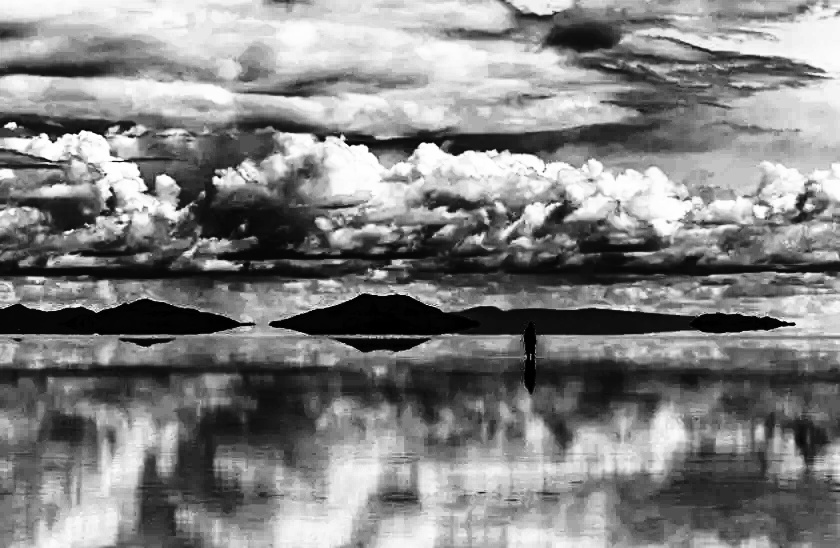
\includegraphics[width=0.9\linewidth]{figure/Q1_equal}
\caption{This figure shows the result of Q1 after histogram equalization.}
\label{fig:q1_equal}
\end{figure}

\begin{figure}[H]
\centering
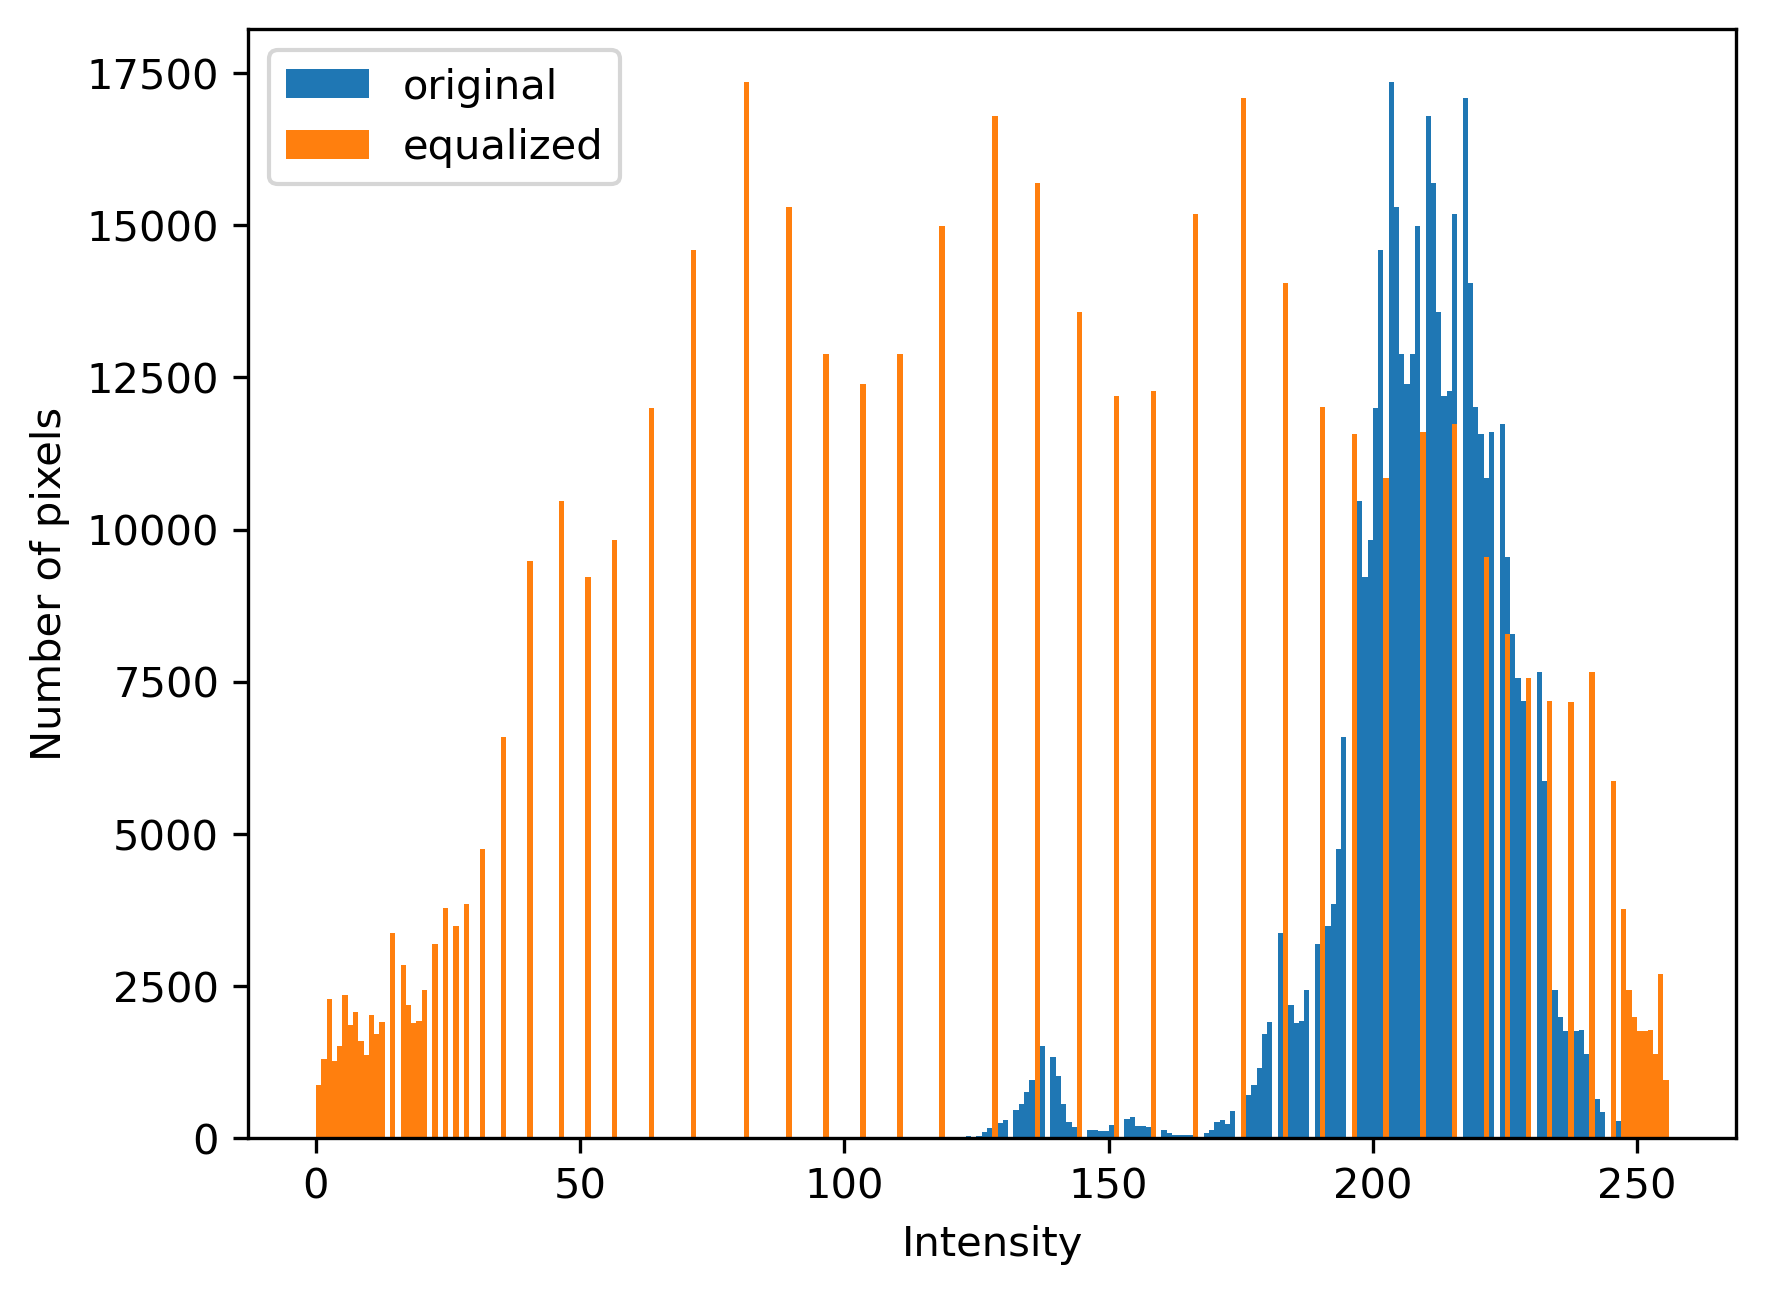
\includegraphics[width=0.9\linewidth]{figure/hist_equal_plt}
\caption{This figure shows the histogram before and after histogram equalization.}
\label{fig:hist_equal_plt}
\end{figure}


\subsection{Histogram Specification}

As we can see in \autoref{fig:q1_spec} and \autoref{fig:hist_match_plt}, because the target image has a high contrast, the contrast of image after histogram specification becomes much higher. 

\begin{figure}[H]
\centering
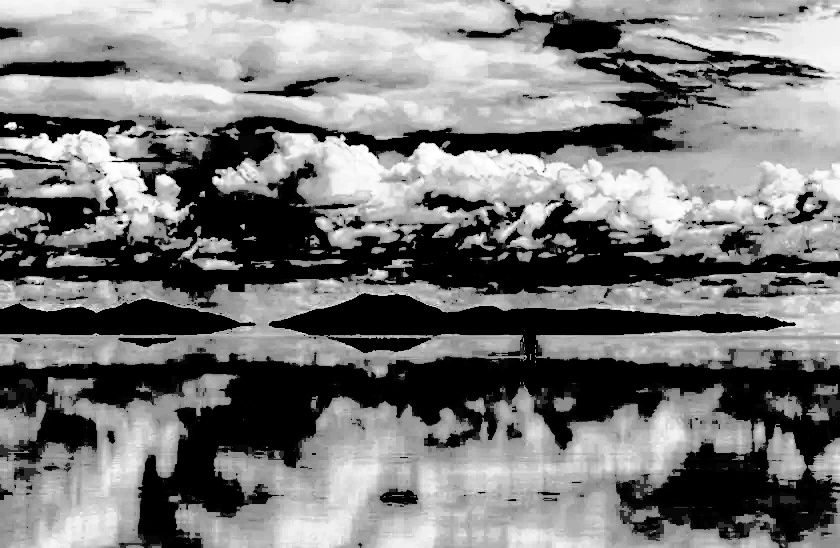
\includegraphics[width=0.9\linewidth]{figure/Q1_spec}
\caption{This figure shows the result of Q1 after histogram equalization.}
\label{fig:q1_spec}
\end{figure}

\begin{figure}[H]
\centering
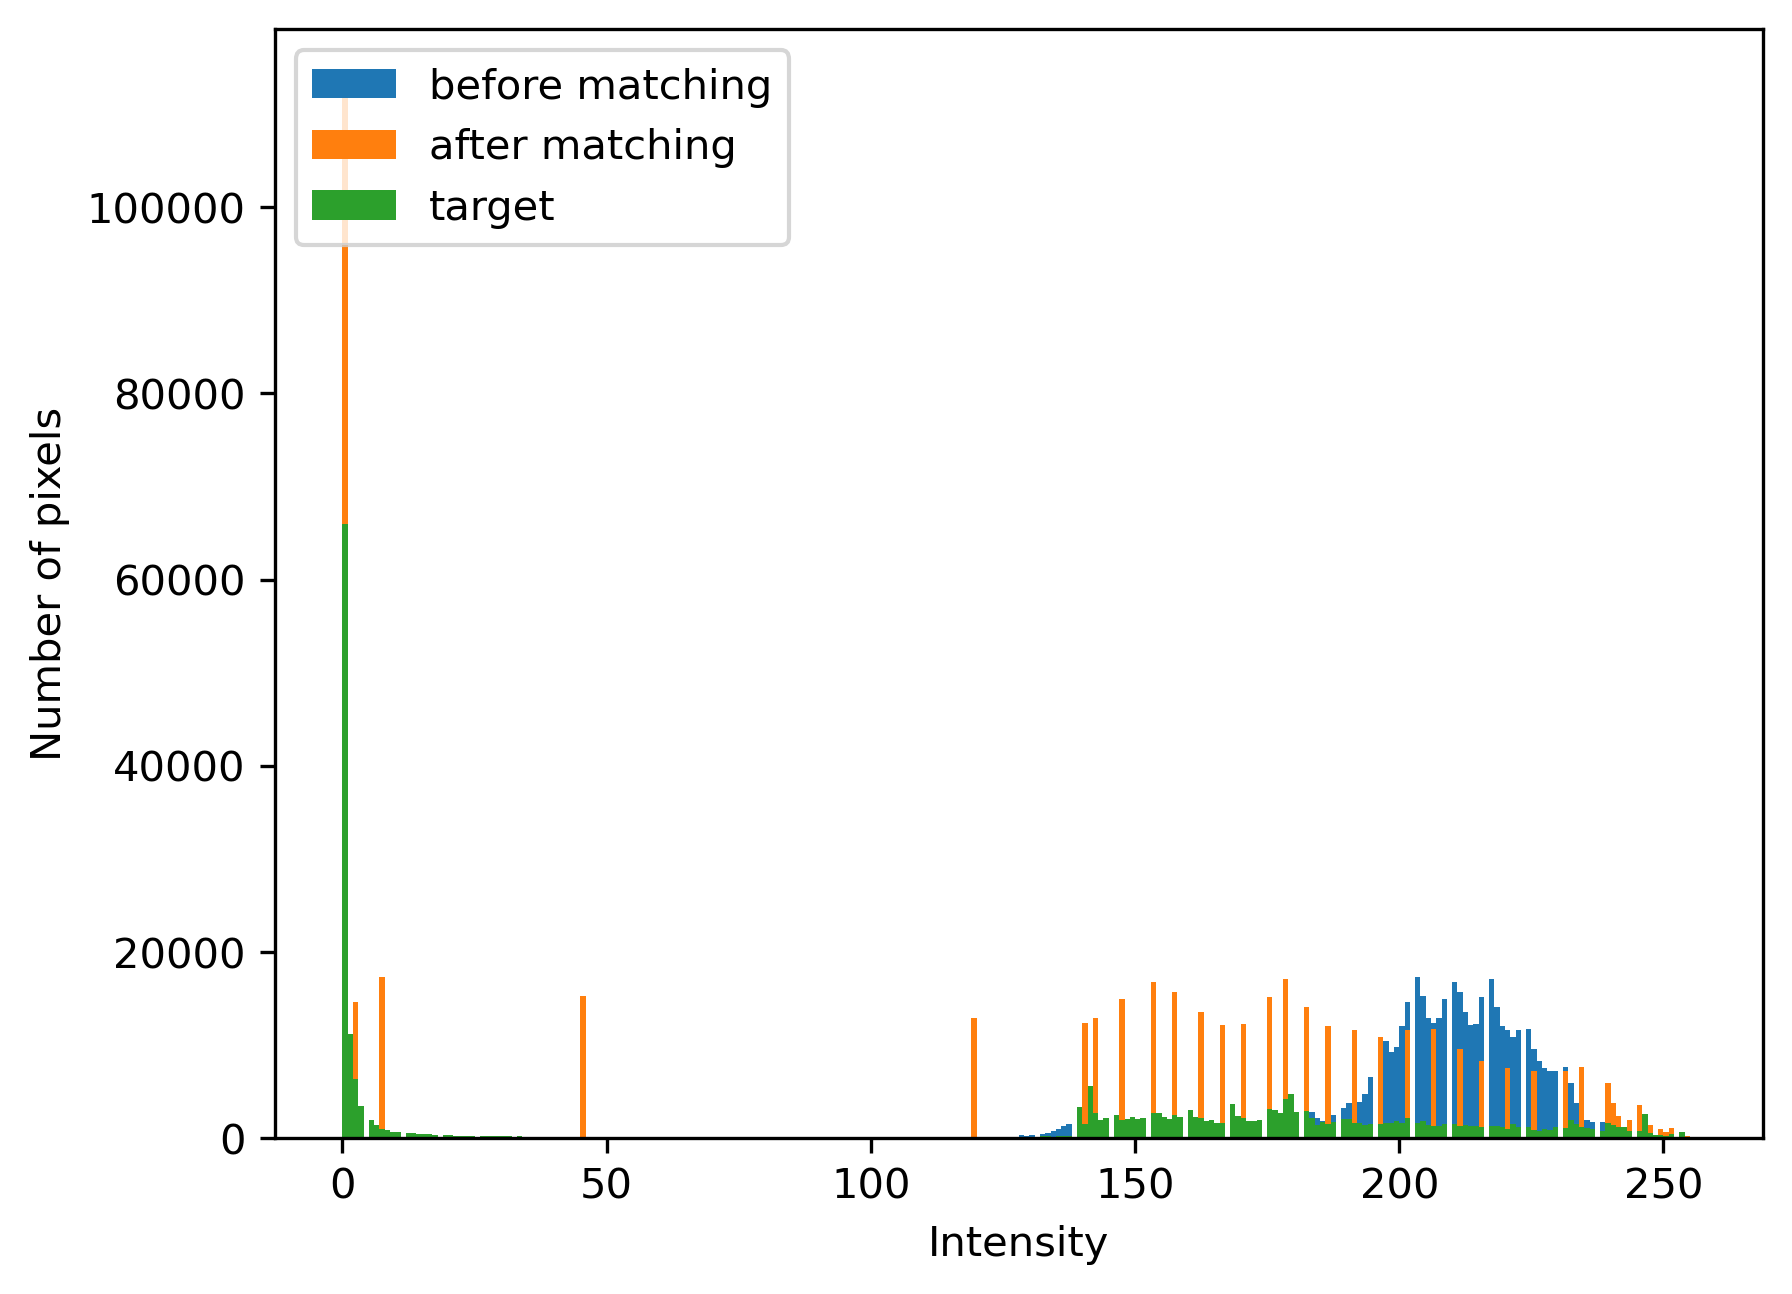
\includegraphics[width=0.9\linewidth]{figure/hist_match_plt}
\caption{This figure shows the histogram before and after histogram specification.}
\label{fig:hist_match_plt}
\end{figure}


\subsection{Gaussian Filter}

The original image, \autoref{fig:before_g} has lots of noises. Therefore, it's a great example to demonstrate the power of Gaussian filter. As we can, the image after applying Gaussian filter, the noises become much lesser, as in \autoref{fig:after_g}.


\begin{figure}[H]
     \centering
     \begin{subfigure}[b]{0.45\linewidth}
         \centering
         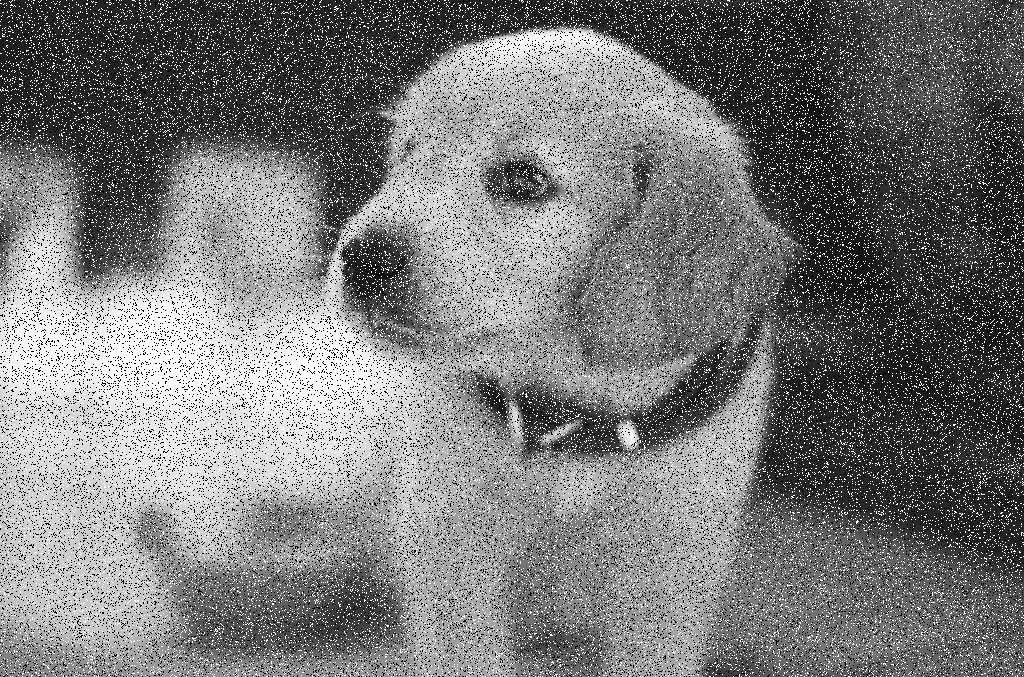
\includegraphics[width=\textwidth]{figure/Q3}
         \caption{Before}
         \label{fig:before_g}
     \end{subfigure}
     \hfill
     \begin{subfigure}[b]{0.45\linewidth}
         \centering
         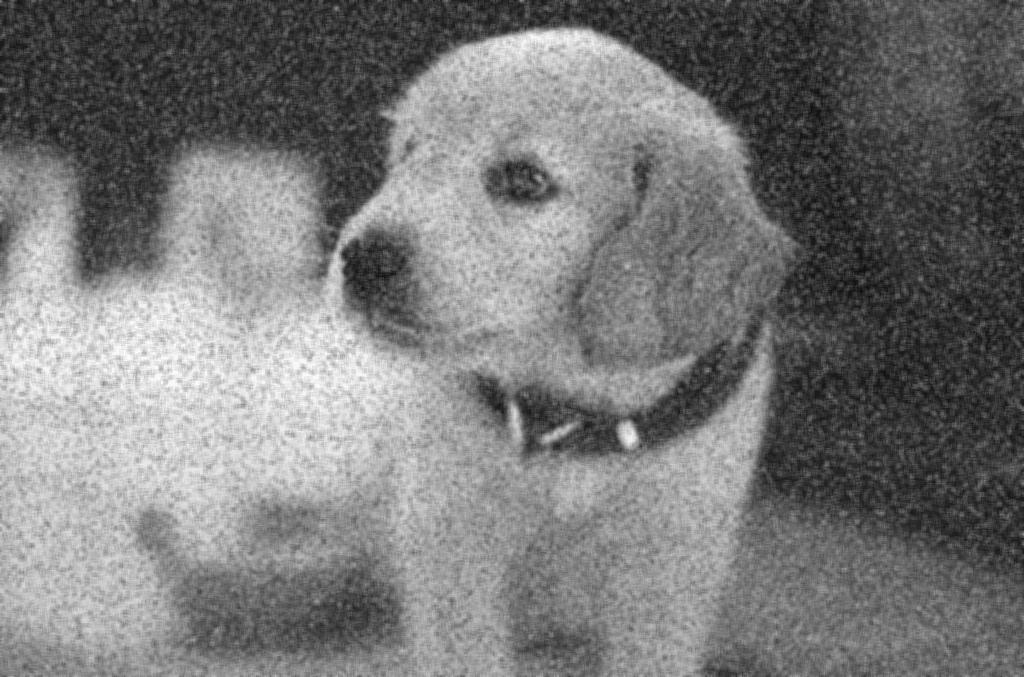
\includegraphics[width=\textwidth]{figure/Q3_gaussian}
         \caption{After}
         \label{fig:after_g}
     \end{subfigure}
        \caption{The comparison of images before and after applying Gaussian filter}
        \label{fig:three graphs}
\end{figure}


\section{Feedback}

In this homework, I learn the basic idea of histogram in image processing, and also understand how the histogram can be used to make the images has different contrast. Changing the contrast of images can make the processing afterward become more effective. 

As for Gaussian filter, because most of the noise in real world follow the Gaussian distribution, using Gaussian filter can remove those noises.


\end{document}